\documentclass[10pt,twocolumn,a4paper]{article}

% ---------- IEEE-style layout (compiles anywhere, no IEEEtran.cls needed) ----------
\usepackage[a4paper,top=19mm,bottom=25mm,left=17mm,right=17mm,columnsep=6mm]{geometry}
\usepackage{mathptmx}
\usepackage[T1]{fontenc}
\usepackage{microtype}
\usepackage{graphicx}
\usepackage{booktabs}
\usepackage{array}
\usepackage{amsmath}
\usepackage[hidelinks]{hyperref}
\usepackage[font=footnotesize,labelsep=period]{caption}
\usepackage{enumitem}
\usepackage{titlesec}
\urlstyle{same}

\renewcommand{\thesection}{\Roman{section}}
\renewcommand{\thesubsection}{\Alph{subsection}}
\titleformat{\section}{\centering\normalsize\scshape}{\thesection.}{0.5em}{}
\titlespacing*{\section}{0pt}{10pt}{5pt}
\titleformat{\subsection}{\normalsize\itshape}{\thesubsection.}{0.5em}{}
\titlespacing*{\subsection}{0pt}{7pt}{3pt}
\captionsetup[table]{labelformat=simple,labelsep=newline,justification=centering,textfont=sc}
\renewcommand{\thetable}{\Roman{table}}
\setlist{nosep,leftmargin=*}
\pagestyle{plain}

\begin{document}

\twocolumn[{%
\begin{center}
{\LARGE Data Centre Power Analysis: Electricity Demand and Clean Supply in Ireland, 2015--2025}\\[5mm]
{\large Roshan Palem}\\[1mm]
{\small Independent Data Analysis Project\\
Dublin, Ireland\\
\href{https://github.com/roshanroy7/data-centre-power-analysis}{github.com/roshanroy7/data-centre-power-analysis}}
\end{center}
\vspace{4mm}
}]

\noindent\textbf{\textit{Abstract}---Data centres are the fastest-growing electricity users in Ireland. This project uses official Central Statistics Office (CSO) and Sustainable Energy Authority of Ireland (SEAI) data to answer three questions: how fast data centre demand is growing, where it is heading by 2030, and whether clean electricity is keeping up. Data centres used 23.2\% of metered electricity in 2025, up from 5.0\% in 2015, a sixfold increase in consumption while all other users grew by about 8\%. Yearly growth peaked at 32\% in 2021 and slowed to about 10\% in 2024 and 2025. Three growth scenarios place the 2030 share between 27\% and 42\%, with a central estimate of about 32\%. Comparing added demand with added wind, solar and hydro output shows that data centres absorbed about 94\% of new clean electricity from 2015 to 2025, and that since 2020 their demand has grown about three times faster than clean supply.}

\section{Introduction}

Ireland has more than 80 data centres, mostly in the Greater Dublin Area, and in 2025 they used nearly as much electricity as every home in the country combined [3]. Their growth matters for two reasons. First, the grid around Dublin is constrained: in 2021 the energy regulator effectively halted standard grid connections for new data centres in the Dublin region [4]. Second, Ireland is committed to moving most of its electricity to renewable sources by 2030. If data centre demand grows faster than clean supply, the gap must be met by gas or imported electricity.

The aim of this project is evidence rather than opinion: a clear, data-backed answer that a decision-maker, such as a government planner, a grid manager or a technology company, could use. The work followed four steps: take the real data, find out what is happening, predict where it is going, and give a recommendation backed by numbers.

The project answers three questions:
\begin{enumerate}
\item How fast is data centre electricity demand really growing?
\item Where is it heading by 2030?
\item Can clean electricity (wind, solar and hydro) keep up?
\end{enumerate}

\section{Data}

Two official datasets were combined (Table~\ref{tab:data}).

\begin{table}[h]
\centering
\caption{Datasets used}
\label{tab:data}
\footnotesize
\begin{tabular}{@{}>{\raggedright\arraybackslash}p{2.9cm}>{\raggedright\arraybackslash}p{2.1cm}>{\raggedright\arraybackslash}p{2.3cm}@{}}
\toprule
Dataset & Coverage & Used for \\
\midrule
CSO MEC02, Data Centres Metered Electricity Consumption [1] & Quarterly, 2015--2025, GWh & Data centre and all other demand \\
\addlinespace
SEAI National Energy Balance [2] & One sheet per year, 2015--2025 (2025 interim), ktoe & Wind, solar and hydro output \\
\bottomrule
\end{tabular}
\end{table}

The CSO table holds 132 values: 44 quarters for three categories (all metered consumption, data centres, and all other customers). The SEAI balance is a 36-sheet workbook with energy flows as rows and fuels as columns, in thousand tonnes of oil equivalent (ktoe). Its column names carry hidden leading spaces, which had to be stripped before the data could be read.

\section{Method}

\subsection{Cleaning and Validation}

The CSO table arrived with three rows per quarter and two columns that were constant in every row. It was pivoted to one row per quarter, the unused columns were dropped, and the categories were renamed. Quarterly shares fluctuate with the seasons, because homes use more electricity in winter and the data centre share dips. This is noise rather than trend, so quarters were summed into calendar years.

Yearly totals were validated against the CSO's published figures. Data centre consumption matched within 1~GWh in every year checked (for example, 6,974 against a published 6,973~GWh for 2024); the gap comes from rounding in the quarterly figures. In the quarters checked, data centres plus other customers equalled the published total, confirming the table was internally consistent.

\subsection{Growth Measures}

For each year the data centre share of total consumption and the year-on-year growth rate were calculated. Both groups were also indexed to 2015 = 100 so their growth could be compared on one scale despite very different sizes. Average growth over the decade was measured as a compound annual growth rate:
\begin{equation}
\text{CAGR} = \left(\frac{V_{2025}}{V_{2015}}\right)^{1/10} - 1
\end{equation}
which gave 20.0\% a year for data centres and 0.8\% for all other users.

\subsection{Scenario Projection}

With only 11 annual observations, a statistical forecasting model would be unreliable, so three transparent scenarios were projected from 2025 actuals (Table~\ref{tab:scen}). Other users were held at their 10-year CAGR of 0.8\% in all scenarios.

\subsection{Clean Electricity}

For each year, the \textit{Indigenous Production} row of the SEAI balance was read for hydro, wind and solar photovoltaic. For these three sources, primary production is electricity, so the values were converted to GWh using 1~ktoe = 11.63~GWh. As a check, 2025 wind came to 12,022~GWh, slightly above the CSO's grid-scale figure of 11,782~GWh [5], as expected because SEAI also counts smaller producers.

\section{Results}

\subsection{Growth of Data Centre Demand}

Data centre consumption rose from 1,240~GWh in 2015 to 7,662~GWh in 2025, and its share of national electricity rose from 5.0\% to 23.2\% (Fig.~\ref{fig:share}).

\begin{figure}[h]
\centering
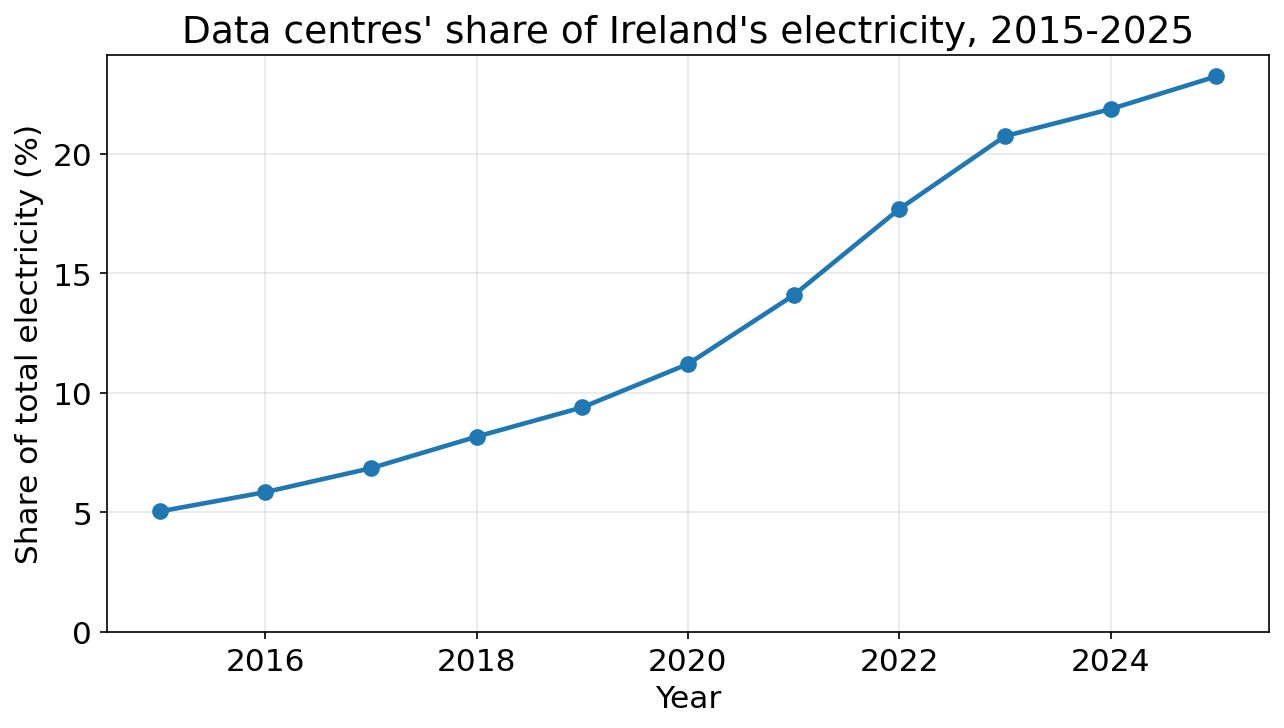
\includegraphics[width=\columnwidth]{figures/01_dc_share.png}
\caption{Data centres' share of Ireland's metered electricity, 2015--2025.}
\label{fig:share}
\end{figure}

Indexed to 2015, data centres reached 618 by 2025, while all other users reached only 108 (Fig.~\ref{fig:index}).

\begin{figure}[h]
\centering
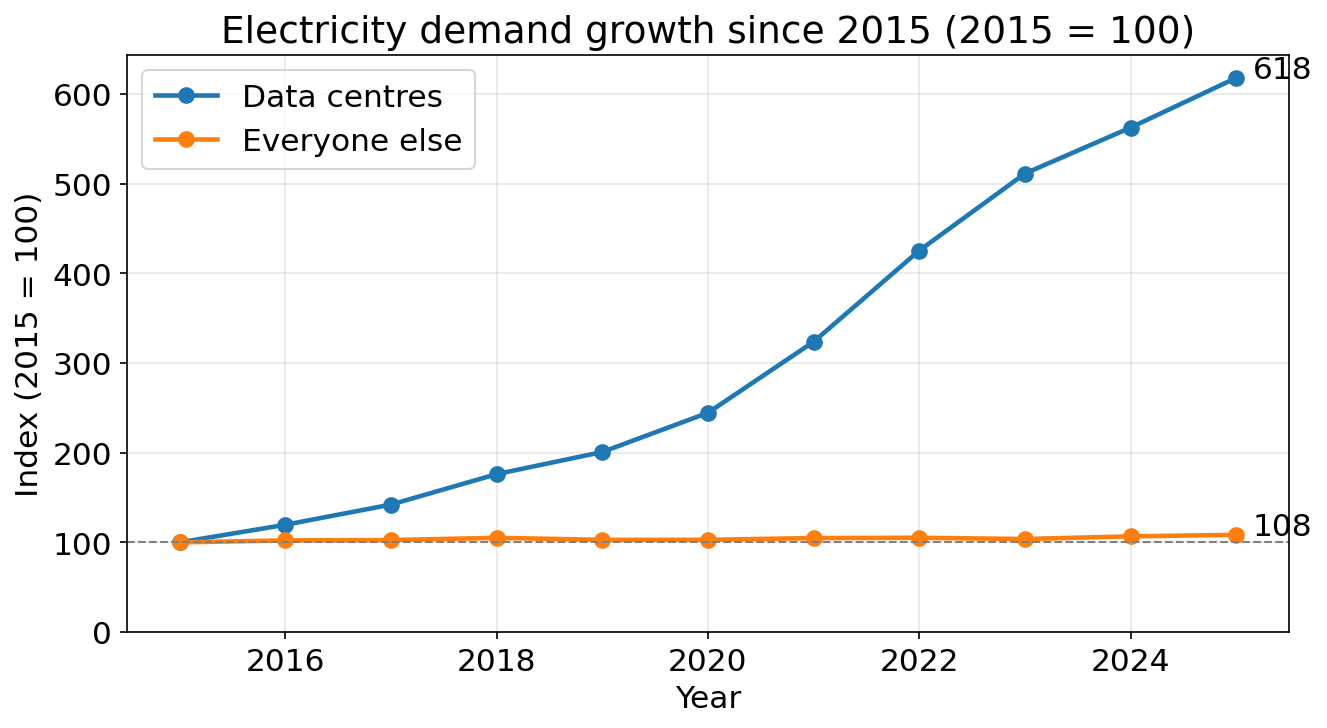
\includegraphics[width=\columnwidth]{figures/02_growth_index.png}
\caption{Growth of electricity demand since 2015 (2015 = 100).}
\label{fig:index}
\end{figure}

Growth is slowing but has not stopped. Yearly data centre growth peaked at 32.4\% in 2021 and 31.4\% in 2022, fell to 20.2\% in 2023, and settled at 10.0\% in 2024 and 9.9\% in 2025. In 2025, data centres still grew about six times faster than other users (1.6\%). The slowdown coincides with the 2021 Dublin connection restrictions, but this data alone cannot show whether the restrictions caused it.

\subsection{Outlook to 2030}

Under the three scenarios, data centres would use between 27\% and 42\% of Ireland's electricity by 2030, with a central estimate of about 32\% (Table~\ref{tab:scen}, Fig.~\ref{fig:scen}).

\begin{table}[h]
\centering
\caption{2030 scenarios}
\label{tab:scen}
\footnotesize
\begin{tabular}{@{}lccc@{}}
\toprule
Scenario & Yearly growth & Basis & 2030 share \\
\midrule
Low & 5\% & Slowdown continues & 27.1\% \\
Central & 10\% & 2024--2025 rate & 31.9\% \\
High & 20\% & 10-year CAGR & 41.9\% \\
\bottomrule
\end{tabular}
\end{table}

\begin{figure}[h]
\centering
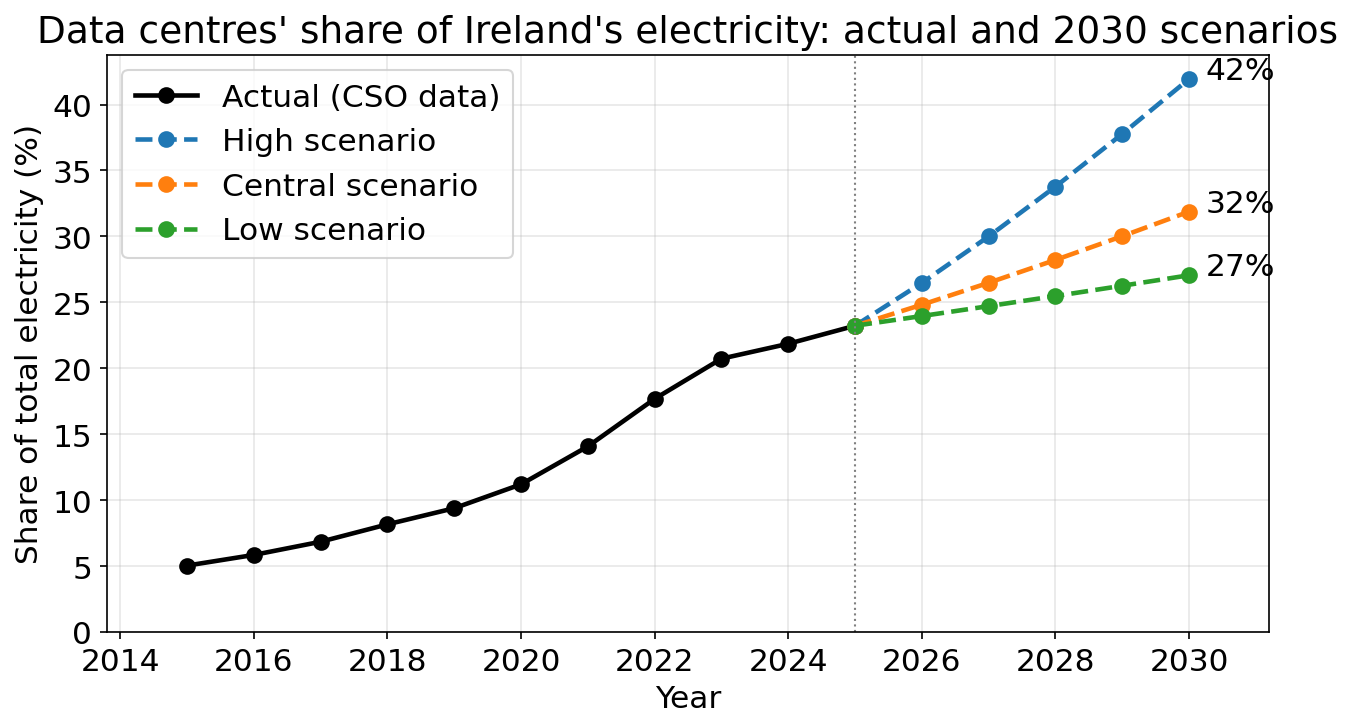
\includegraphics[width=\columnwidth]{figures/03_scenarios_2030.png}
\caption{Actual data centre share and three projections to 2030.}
\label{fig:scen}
\end{figure}

The central estimate lies between two official views. The energy regulator projects about 31\% by 2034 [6], four years later than the central scenario. In 2024 the International Energy Agency warned of about a third by 2026 [4], which has not happened: the share was 23\% in 2025.

\subsection{Clean Electricity Against Data Centre Demand}

Table~\ref{tab:clean} compares the growth in clean electricity with the growth in data centre demand over two periods.

\begin{table}[h]
\centering
\caption{Added clean supply and added data centre demand}
\label{tab:clean}
\footnotesize
\begin{tabular}{@{}lcc@{}}
\toprule
Period & Clean electricity added & Data centre demand added \\
\midrule
2015--2025 & 6,814 GWh & 6,422 GWh \\
2020--2025 & 1,575 GWh & 4,631 GWh \\
\bottomrule
\end{tabular}
\end{table}

Over the full decade, data centres absorbed about 94\% of all new clean electricity. Since 2020 the picture is worse: data centre demand grew about three times faster than clean supply. Until 2020, clean supply grew well ahead of data centre demand, by about 3,400~GWh. Since then wind output has been almost flat (11,742~GWh in 2020, 12,022~GWh in 2025), and by 2025 the lead had shrunk to about 400~GWh (Fig.~\ref{fig:clean}).

\begin{figure}[h]
\centering
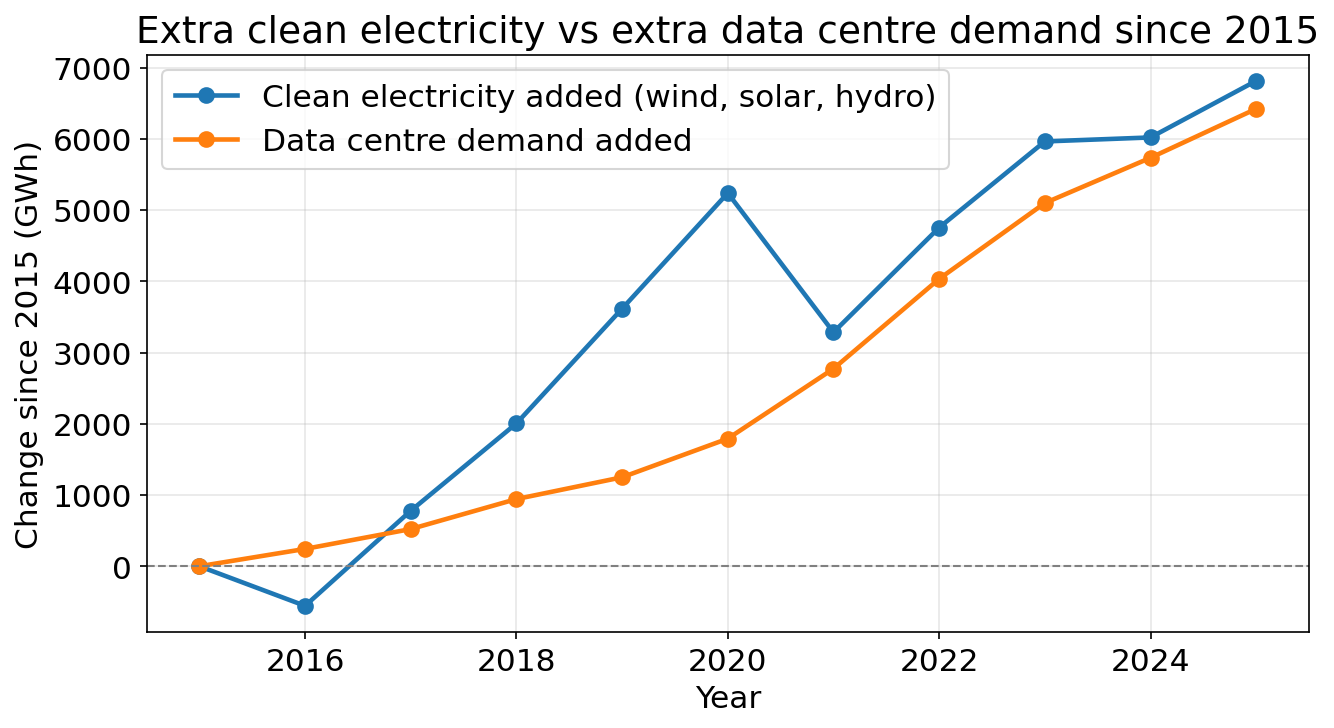
\includegraphics[width=\columnwidth]{figures/04_clean_vs_dc.png}
\caption{Cumulative change since 2015 in clean electricity (wind, solar, hydro) and in data centre demand.}
\label{fig:clean}
\end{figure}

Data centre demand rises smoothly every year, while clean supply swings with the weather, falling in low-wind years such as 2016 and 2021. A steady demand covered by an unsteady supply explains why gas and imported electricity remain necessary; in 2025, Ireland imported 16.3\% of its electricity supply [2].

\section{Limitations}

\begin{itemize}
\item \textbf{Short history.} Eleven years of data is thin for forecasting; the scenarios show a range, not a prediction.
\item \textbf{Other users.} The projection holds other users at 0.8\% growth a year. Wider use of electric cars and heat pumps would raise this and lower the data centre share.
\item \textbf{Shared grid.} Data centres do not draw on specific sources. Section IV-C compares added demand with added clean supply as an accounting exercise; it makes no claim about which source powers data centres.
\item \textbf{Weather.} Wind output varies from year to year. 2020 was a windy year, which raises the 2020 baseline.
\item \textbf{Two sources.} Demand comes from the CSO and supply from SEAI, and SEAI's 2025 figures are provisional.
\item \textbf{Scope of clean supply.} Biomass and other bio-renewables are excluded, so clean supply is slightly understated.
\end{itemize}

\section{Conclusions and Future Work}

Data centre demand in Ireland is growing more slowly than in 2021 and 2022, but it still rises every year and has outpaced new clean electricity since 2020. If current trends continue, data centres will use around a third of national electricity by 2030, and unless wind and solar build-out speeds up, more of the extra demand will be met by gas and imports.

Future work could add biomass and other renewables to the clean supply measure, model faster growth in other demand from electrification, use monthly data to study seasonal pressure on the grid, and present the results in an interactive dashboard.

\section*{References}
\footnotesize\raggedright
\begin{enumerate}[label={[\arabic*]},leftmargin=*]
\item Central Statistics Office, ``Data Centres Metered Electricity Consumption 2025,'' table MEC02, Jul. 2026. \url{https://www.cso.ie/en/releasesandpublications/ep/p-dcmec/datacentresmeteredelectricityconsumption2025/}
\item Sustainable Energy Authority of Ireland, ``National Energy Balance,'' 2025 interim, May 2026. \url{https://www.seai.ie/resources/seai-statistics/key-publications/national-energy-balance/}
\item ITPro, ``Data centers gobbled up 23 percent of Ireland's electricity supply in 2025,'' 2026.
\item Computing, ``Ireland's datacentres now consume nearly a quarter of nation's electricity,'' 2026.
\item EirGrid, ``42\% of electricity came from renewable sources in September,'' Oct. 2025.
\item eWeek, ``Irish data centers used 23\% of national electricity in 2025,'' 2026.
\end{enumerate}

\end{document}
